% !TeX root = surprises.tex

\chapter{מחוגה מתמוטטת}\label{c.collapse}

%%%%%%%%%%%%%%%%%%%%%%%%%%%%%%%%%%%%%%%%%%%%%%%%%%%%%%%%%%%%%%%

במחוגה מודרנית היא 
\textbf{מחוגה קבועה}:
ניתן לקבע את המרחק בין שתי הרגליים וכך להעתיק קטע קו או מעגל ממקום למקום (%
\ref{fig.fixed-compass}).
אוקלידס השתמש במחוגה 
\textbf{מתמוטטת}
\L{(collapsing)}
בה לא ניתן לשמור מרחק קבוע (%
\ref{fig.collapsing-compass}).
שרגליה מתקפלות כאשר מרימים אותן מהנייר. לעתים קרובות מורים משתמשים מחוגה מתמוטטת המורכבת מטוש שמחובר לחוט כדי לבנות מעגל הלוח. אי-אפשר לשמור על מרחק קבוע כאשר מרימים את המחוגה מהלוח.

\begin{figure}[tb]
\begin{center}
\begin{subfigure}{.4\textwidth}
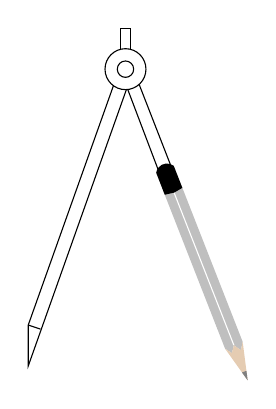
\begin{tikzpicture}
\begin{scope}[rotate=0,transform shape,scale=2.6]
\draw (2.95,3.7) rectangle (3,3.95);
\draw (2.92,3.68) -- (2.5,2.5) -- (2.5,2.3) -- (2.99,3.68);
\draw (3.5,2.5) -- (3.43,2.48) -- (2.975,3.68);
\draw (3.04,3.68) -- (3.5,2.5);
\draw (2.5,2.5) -- (2.56,2.48);
\draw[fill=white] (2.975,3.75) circle (0.1cm);
\draw (2.975,3.75) circle (0.04cm);
\end{scope}
\begin{scope}[xshift=9cm,yshift=6.2cm,rotate=21.4,scale=.6]          
\fill[gray!50] (0,4) -- (0.4,4) -- (0.4,0) --
               (0.3,-0.15) -- (0.2,0) -- (0.1,-0.14) --
               (0,0) -- cycle;
\draw[color=white] (0.2,4) -- (0.2,0);
\fill[black] (0,3.5) -- (0.2,3.47) -- (0.4,3.5) --
             (0.4,4) arc(30:150:0.23cm);
\fill[brown!40] (0,0) -- (0.2,-0.8)
    node[coordinate,pos=0.75](a){} -- 
    (0.4,0)node[coordinate,pos=0.25](b){} -- 
    (0.3,-0.15) -- (0.2,0) -- (0.1,-0.14) -- cycle;
\fill[gray] (a) -- (0.2,-0.8) -- (b) -- cycle;
\end{scope}
\end{tikzpicture}
\selectlanguage{hebrew}
\caption{מחוגה קבועה. לרגל אחת סיכה שניתן להניח במרכז המעגל. עפרון מחוברת לרגל השניה משמש לשרטוט המעגל. הרגלים מחוברות בציר קשיח כך שהמרחק בין הרגליים (רדיוס המעגל) נשמר גם כאשר מרימים את המחוגה מהנייר.}
\label{fig.fixed-compass}
\end{subfigure}
\hspace{3em}
\begin{subfigure}[b]{.4\textwidth}
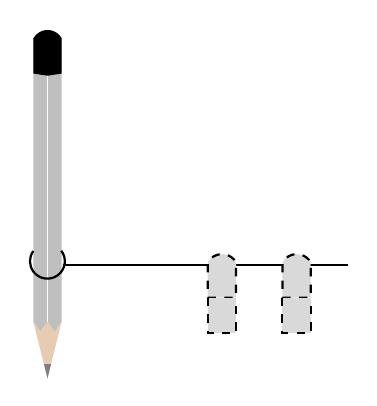
\begin{tikzpicture}[rotate=0,scale=.9]          
\fill[gray!50] (0,4) -- (0.4,4) -- (0.4,0) --
               (0.3,-0.15) -- (0.2,0) -- (0.1,-0.14) --
               (0,0) -- cycle;
\draw[color=white] (0.2,4) -- (0.2,0);
\fill[black] (0,3.5) -- (0.2,3.47) -- (0.4,3.5) --
             (0.4,4) arc(30:150:0.23cm);
\fill[brown!40] (0,0) -- (0.2,-0.8)
    node[coordinate,pos=0.75](a){} -- 
    (0.4,0) node[coordinate,pos=0.25](b){} -- 
    (0.3,-0.15) -- (0.2,0) -- (0.1,-0.14) -- cycle;
\fill[gray] (a) -- (0.2,-0.8) -- (b) -- cycle;

\draw[thick] (0.395,1) arc (37:-216:7pt);
\coordinate (knot) at (0.44,.8);
\draw[thick] (knot) -- +(4,0);
\fill (knot) circle (.7pt);

\begin{scope}[xshift=100pt,yshift=-90pt]
\draw[dashed,thick,fill=white!70!gray] (0,3.5) -- (0.4,3.5) -- 
      (0.4,4) arc(30:150:0.23cm) -- cycle;
\draw[dashed,thick,fill=white!70!gray] (0,3.5) -- ++(0,-.5) -- ++(.4,0) -- ++(0,.5);
\end{scope}

\begin{scope}[xshift=70pt,yshift=-90pt]
\draw[dashed,thick,fill=white!70!gray] (0,3.5) -- (0.4,3.5) -- 
      (0.4,4) arc(30:150:0.23cm) -- cycle;
\draw[dashed,thick,fill=white!70!gray] (0,3.5) -- ++(0,-.5) -- ++(.4,0) -- ++(0,.5);
\end{scope}
\end{tikzpicture}
\selectlanguage{hebrew}
\caption{%
מחוגה מתמוטטת. המשתמש מצמיד חוט למרכז המעגל. לקצה השני של החוט מחובר עפרון המשמש לשרטוט המעגל. כאשר מרימים את המחוגה מהנייר, האצבעות (מקווקווים) יכולים בקלות להחליק למקום אחר.%
}\label{fig.collapsing-compass}
\end{subfigure}
\end{center}
\end{figure}

בתחילת הפרק דיון על הרלוונטית של למידה של בנייה עם סרגל ומחוגה (סעיף%
~\ref{s.relevance}).
סעיף%
~\ref{s.collapse} 
משווה את שני סוגי המחוגה בבנייה הפשוטה ביותר: אנך אמצעי. סעיף%
~\ref{s.collapse-copy}
מביא את השיטה של אוקלידס להעתקת קטע קו באמצעות מחוגה מתמוטטת. זה מוכיח שניתן לבצע באמצעות מחוגה מתמוטטת כל בנייה שניתנת לביצוע באמצעות מחוגה קבועה. סעיף%
~\ref{s.collapse-copy-incorrect} 
מציג הוכחה של משפט זה שנראית נכונה אבל היא לא נכונה עבור כל תצורה של קווים ונקודות. כדי להדגיש שאין לסמוך על שרטוט, סעיף%
~\ref{s.collapse-isoceles}
מביא "הוכחה לכאורה" מפורסמת שכל משולש הוא שווי שוקיים. ההוכחה נראית נכונה אבל היא שגויה כי היא מתבססת על שרטוט לא נכון.

%%%%%%%%%%%%%%%%%%%%%%%%%%%%%%%%%%%%%%%%%%%%%%%%%%%%%%%%%%%%%%%

\section{בנייה עם סרגל ומחוגה}\label{s.relevance}

עד לאחרונה בנייה עם סרגל ומחוגה היתה המושג הבסיסי שנלמד בגיאומטריה אוקלידית, אולם חשיבותה ירדה בסילבוסים מודרניים. מובן שלנושא אין כמעט חשיבות מעשיות. כפי שאנו מראים בסעיפים%
~\ref{s.neusis}, \ref{s.neusis-doubling}, \ref{s.q}, \ref{s.square-quad},
היוונים ידעו לבנות בניות שאינן אפשריות עם סרגל ומחוגה באמצעות כליםי שהם רק מעט מתקדמים יותר. היום מחשבים מסוגלים לבצע בניות בדיוק רב כלל שנרצה באמצעות חישובים נומריים.

למרות זאת, אני מאמין שיש יתרונות ללמוד בניות עם סרגל ומחוגה:
\begin{itemize}
\item
מעניין יותר ומאתגר יותר ללמוד גיאומטריה דרך בניות לעומת קריאה של משפטים והוכחות.
\item
התקדמויות מכריעות במתמטיקה הושגו במסגרת נסיונות למצוא בניות. פרק%
~\ref{c.heptadecagon}
מביא בנייה של 
\L{Gauss}
שהיתה נקודת מוצא של אלגברה מודרנית, במיוחד התיאוריה שפותחה על יד 
\L{\'{E}variste Galois}.
\item
העובדה שיש בניות שאינן אפשריות קשה לעיכול ולכן מאוד מעניין.
\item
מעציב שאנשים רבים מבזבזים שנים של חייהם בניסיון לבצע בניות שאינן אפשריות. חשוב שתלמידים יכירו שהמאמצים הללו חסרי תוחלת.
\end{itemize}


%%%%%%%%%%%%%%%%%%%%%%%%%%%%%%%%%%%%%%%%%%%%%%%%%%%%%%%%%%%%%%%

\section{מחוגה קבועה ומחוגה מתמוטטת}\label{s.collapse}

בספרי לימוד גיאומטריה ניתן למצוא בנייה של אנך אמצעי לקטע קו על ידי בניית שני מעגלים שמרכזם על הקו,ובלבד שהרדיוס גדול ממחצית המרחק בין המרכזים 
(\ref{f.collapse-perp-bisector-fixed}).
בנייה זו אפשרית רק עם מחוגה קבועה כי לאחר בניית המעגל שמרכזו 
$A$,
המרחק בין רגלי המחוגה חייב להישאר ללא שינוי כדי לבנותאת המעגל שמרכזו 
$B$.

\ref{f.collapse-perp-bisector-collapse}
מראה בנייה של אנך אמצעי שפועלת גם עם מחוגה קבועה וגם עם מחוגה מתמוטטת. נבנה שני מעגלים: אחד שמרכזו 
$A$
עם רדיוס
$\overline{AB}$
ואחד עם רדיוס
$\overline{BA}$.
הבנייה אפשרית עם מחוגה מתמוטטת כי (ברור)
$\overline{AB}=\overline{BA}$,
ולכן המחוגה לא חייבת "לזכור" את האורך של
$\overline{AB}$
כדי לבנות מעגל שמרכזו 
$B$
עם רדיוס זהה.

הוכחת הנכונות של הבנייה ב-%
\ref{f.collapse-perp-bisector-fixed}
לא פשוטה בכלל כי חייבים להשתמש במושגים יחסית מתקדמים כגון משולשים חופפים. אבל הוכחת הנכונות של הבנייה ב-%
\ref{f.collapse-perp-bisector-collapse}
פשוטה ומבוססת על העובדה ש-%
$\triangle ABC$
הוא משולש שווה-צלעות. טענה זו היא המשפט הראשון בספר של אוקלידס. 
$\overline{AC}=\overline{AB}$
כי הם רדיוסים של אותו מעגל, וכן
$\overline{BC}=\overline{BA}$.
מכאן:
$\overline{AC} = \overline{AB} = \overline{BA} = \overline{BC}$.

\ref{f.collapse-equilateral-fixed}
מראה שעבור הבנייה עם מחוגה קבועה, המשולש יהיה שווה-שוקיים, לא בהכרח שווה-צלעות 
(\ref{f.collapse-equilateral-collapse}).

%%%%%%%%%%%%%%%%%%%%%%%%%%%%%%%%%%%%%%%%%%%%%%%%%%%%%%%%%%%%%%%


\section{העתקת קטע קו לפי אוקלידס}\label{s.collapse-copy}

המשפט השני של ספרו של אוקלידס מתאר איך להעתיק קטע קו נתון
$\overline{AB}$
לקטע באותו אורך שאחת מנקודות הקצה שלו היא נקודה נתונה
$C$.
מכאן שמחוגה קבועה לא מוסיף יכולות ואפשר להסתפק במחוגה מתמוטטת, אבל הבניות יהיו מסובכות יותר.

\begin{theorem}
נתון קטע קו
$\overline{AB}$
ונקודה
$C$,
ניתן לבנות עם מחוגה מתמוטטת בנקודה
$C$,
ניתן לבניות עם מחוגה מתמוטטת קטע קו
$\overline{CC'}$
שאחת מנקודות הקצה שלו הוא
$C$
ואורכו
$\overline{AB}=\overline{CC'}$ (\ref{f.collapse-copying-1}).
\end{theorem}

\begin{figure}[tb]
\begin{center}
\begin{subfigure}{.4\textwidth}
\begin{tikzpicture}[scale=0.5]
\coordinate (A) at (0,0);
\coordinate (B) at (4,0);
\vertex{A};
\vertex{B};
\draw (A) node[below left] {$A$} -- (B) node[below right] {$B$};
\draw[name path=larc] (A) ++(-60:3cm) arc (-60:60:3cm);
\draw[name path=rarc] (B) ++(-120:3cm) arc (-120:-240:3cm);
\path [name intersections={of=larc and rarc,by={b,t}}];
\node[above right,xshift=-2pt,yshift=5pt] at (t) {$C$};
\node[below left,xshift=2pt,yshift=-5pt] at (b) {$D$};
\draw ($ (b) ! 1.2 ! (t)$) -- ($ (t) ! 1.2 ! (b)$);
\end{tikzpicture}
\selectlanguage{hebrew}
\caption{בניית חוצה אנכי עם מחוגה קבועי}\label{f.collapse-perp-bisector-fixed}
\end{subfigure}
\hfill
\begin{subfigure}{.4\textwidth}
\begin{tikzpicture}[scale=0.5]
\coordinate (A) at (0,0);
\coordinate (B) at (4,0);
\vertex{A};
\vertex{B};
\draw (A) node[below left] {$A$} -- (B) node[below right] {$B$};
\draw[name path=larc] (A) ++(-80:4cm) arc (-80:80:4cm);
\draw[name path=rarc] (B) ++(-100:4cm) arc (-100:-260:4cm);
\path [name intersections={of=larc and rarc,by={b,t}}];
\node[above right,xshift=-2pt,yshift=3pt] at (t) {$C$};
\node[below left,xshift=2pt,yshift=-3pt] at (b) {$D$};
\draw ($ (b) ! 1.2 ! (t)$) -- ($ (t) ! 1.2 ! (b)$);
\end{tikzpicture}
\selectlanguage{hebrew}
\caption{בניית חוצה אנכי עם מוחגה מתמוטטת}\label{f.collapse-perp-bisector-collapse}
\end{subfigure}
\end{center}
\end{figure}


\begin{figure}[tb]
\begin{center}
\begin{subfigure}{.4\textwidth}
\begin{tikzpicture}[scale=0.5]
\coordinate (A) at (0,0);
\coordinate (B) at (4,0);
\vertex{A};
\vertex{B};
\draw (A) node[below left] {$A$} -- (B) node[below right] {$B$};
\draw[name path=larc] (A) ++(-60:3cm) arc (-60:60:3cm);
\draw[name path=rarc] (B) ++(-120:3cm) arc (-120:-240:3cm);
\path [name intersections={of=larc and rarc,by={b,t}}];
\vertex{t};
\vertex{b};
\node[above right,xshift=-2pt,yshift=5pt] at (t) {$C$};
\node[below left,xshift=2pt,yshift=-5pt] at (b) {$D$};
\draw (A) -- (t);
\draw (B) -- (t);
\end{tikzpicture}
\selectlanguage{hebrew}
\caption{בניית משולש שווה-שוקיים עם מחוגה קבועה}\label{f.collapse-equilateral-fixed}
\end{subfigure}
\hspace{3em}
\begin{subfigure}{.4\textwidth}
\begin{tikzpicture}[scale=0.5]
\coordinate (A) at (0,0);
\coordinate (B) at (4,0);
\draw (A) node[below left] {$A$} -- (B) node[below right] {$B$};
\vertex{A};
\vertex{B};
\draw[name path=larc] (A) ++(-80:4cm) arc (-80:80:4cm);
\draw[name path=rarc] (B) ++(-100:4cm) arc (-100:-260:4cm);
\path [name intersections={of=larc and rarc,by={b,t}}];
\vertex{t};
\vertex{b};
\node[above right,xshift=-2pt,yshift=3pt] at (t) {$C$};
\node[below left,xshift=2pt,yshift=-3pt] at (b) {$D$};
\draw (A) -- (t);
\draw (B) -- (t);
\end{tikzpicture}
\selectlanguage{hebrew}
\caption{בניית משולש שווה-צלעות עם מחוגה מתמוטטת}\label{f.collapse-equilateral-collapse}
\end{subfigure}
\end{center}
\end{figure}

\begin{figure}[tb]
\begin{center}
\begin{subfigure}{.4\textwidth}
\begin{tikzpicture}[scale=0.5]
\coordinate (C) at (0,0);
\coordinate (A) at (3,0);
\draw (A) node[below,xshift=-2pt,yshift=-2pt] {$A$} -- +(40:4) coordinate (B) node[right] {$B$};
\vertex{A};
\vertex{B};
\vertex{C};
\node[below,xshift=2pt,yshift=-2pt] at (C) {$C$};
\draw[thick,dashed] (C) -- +(160:4) coordinate (D) node[below] {$C'$};
\vertex{D};
\end{tikzpicture}
\selectlanguage{hebrew}
\caption{העתקת קטע קו$\overline{AB}$; אין חשיבות לכיוון של $\overline{CC'}$}\label{f.collapse-copying-1}
\end{subfigure}
\hspace{3ex}
\begin{subfigure}{.4\textwidth}
\begin{tikzpicture}[scale=0.5]
\coordinate (C) at (0,0);
\coordinate (A) at (3,0);
\draw (A) node[below,xshift=-2pt,yshift=-2pt] {$A$} -- +(40:4) coordinate (B) node[right] {$B$};
\vertex{B};
\node[below,xshift=2pt,yshift=-2pt] at (C) {$C$};
\draw (A) -- (C);
\path[name path=larc] (C) ++(-70:2.5cm) arc (-70:70:2.5cm);
\path[name path=rarc] (A) ++(-110:2.5cm) arc (-110:-250:2.5cm);
\path [name intersections={of=larc and rarc,by={d,D}}];
\node[above] at (D) {$D$};
\draw (A) -- (D);
\draw (C) -- (D);
\end{tikzpicture}
\selectlanguage{hebrew}
\caption{העתקת קו עם מחוגה מתמוטטת}\label{f.collapse-copying-2}
\end{subfigure}
\end{center}
\end{figure}

\begin{proof}
נבנה קטע קו
$\overline{AC}$
ומשולש שווה-צלעות 
$\triangle ACD$
שבסיסו
$\overline{AC}$
(\ref{f.collapse-copying-2}).
לפי המשפט הראשון של אוקלידס הבנייה אפשרית באמצעות מחוגה מתמוטטת. נבנה קרן שהיא המשך של קטע הקו מ-%
$D$
לכיוון 
$A$,
ונבנה קרן שהיא המשך של 
$D$
לכיוון
$C$
(\ref{f.collapse-copying-3}).

נבנה מעגל שמרכזו 
$A$
עם רדיוס
$\overline{AB}$,
ונסמן ב-%
$E$
את נקודת החיתוך של המעגל עם הקרן שממשיכה את
$\overline{DA}$
(\ref{f.collapse-copying-4}).
נבנה מעגל שמרכזו 
$D$
עם רדיוס 
$\overline{DE}$,
ונסמן ב-%
$F$
את נקודת החיתוך של המעגל עם הקרן שממשיכה את
$\overline{DC}$
(איור%
\ref{f.collapse-copying-5}).

\begin{figure}[tb]
\begin{center}
\begin{subfigure}{.4\textwidth}
\begin{tikzpicture}[scale=0.6]
\coordinate (C) at (0,0);
\coordinate (A) at (2.5,0);
\coordinate (B) at (5.5,2);
\draw (A) node[below,xshift=-2pt,yshift=-2pt] {$A$} -- (B) node[right] {$B$};
%\fill (A) circle[radius=3pt];
%\fill (B) circle[radius=3pt];
\node[below,xshift=2pt,yshift=-2pt] at (C) {$C$};
\draw (A) -- (C);
\path[name path=larc] (C) ++(-70:2.5cm) arc (-70:70:2.5cm);
\path[name path=rarc] (A) ++(-110:2.5cm) arc (-110:-250:2.5cm);
\path [name intersections={of=larc and rarc,by={d,D}}];
\node[above] at (D) {$D$};
\draw (A) -- (D);
\draw (C) -- (D);
\draw[name path=ray2] (D) -- ($ (D) ! 2.7 ! (C) $);
\draw[name path=ray1] (D) -- ($ (D) ! 2.7 ! (A) $);
\end{tikzpicture}
\selectlanguage{hebrew}
\caption{בניית קרניים מ-%
$D$}\label{f.collapse-copying-3}
\end{subfigure}
\hspace{3ex}
\begin{subfigure}{.4\textwidth}
\begin{tikzpicture}[scale=0.6]
\coordinate (C) at (0,0);
\coordinate (A) at (2.5,0);
\coordinate (B) at (5.5,2);
\draw (A) node[below,xshift=-2pt,yshift=-2pt] {$A$} -- (B) node[right] {$B$};
%\fill (A) circle[radius=3pt];
%\fill (B) circle[radius=3pt];
%\fill (C) node[below,xshift=2pt,yshift=-2pt] {$C$} circle[radius=3pt];
\node[below,xshift=2pt,yshift=-2pt] at (C) {$C$};
\draw (A) -- (C);
\path[name path=larc] (C) ++(-70:2.5cm) arc (-70:70:2.5cm);
\path[name path=rarc] (A) ++(-110:2.5cm) arc (-110:-250:2.5cm);
\path [name intersections={of=larc and rarc,by={d,D}}];
%\fill (D) node[above] {$D$} circle[radius=3pt];
\node[above] at (D) {$D$};
\draw (A) -- (D);
\draw (C) -- (D);
\draw[name path=ray2] (D) -- ($ (D) ! 2.7 ! (C) $);
\draw[name path=ray1] (D) -- ($ (D) ! 2.7 ! (A) $);
\node[draw,circle through=(B),name path=c1] at (A) {};
\path [name intersections={of=c1 and ray1,by={E,e}}];
%\fill (E) node[right,xshift=2pt,yshift=-2pt] {$E$} circle[radius=3pt];
\node[right,xshift=2pt,yshift=-2pt] at (E) {$E$};
\end{tikzpicture}
\selectlanguage{hebrew}
\caption{בניית מעגל עם רדיוס 
$\overline{AB}$}\label{f.collapse-copying-4}
\end{subfigure}
\end{center}
\end{figure}

\begin{figure}[tb]
\begin{center}
\begin{tikzpicture}[scale=0.4]
\coordinate (C) at (0,0);
\coordinate (A) at (2.5,0);
\coordinate (B) at (5.5,2);
\draw (A) node[below,xshift=-2pt,yshift=-2pt] {$A$} -- (B) node[right] {$B$};
%\fill (A) circle[radius=3pt];
%\fill (B) circle[radius=3pt];
%\fill (C) node[below,xshift=2pt,yshift=-2pt] {$C$} circle[radius=3pt];
\node[below,xshift=2pt,yshift=-2pt] at (C) {$C$};
\draw (A) -- (C);
\path[name path=larc] (C) ++(-70:2.5cm) arc (-70:70:2.5cm);
\path[name path=rarc] (A) ++(-110:2.5cm) arc (-110:-250:2.5cm);
\path [name intersections={of=larc and rarc,by={d,D}}];
%\fill (D) node[above] {$D$} circle[radius=3pt];
\node[above] at (D) {$D$};
\draw (A) --  (D);
\draw (C) --  (D);
\draw[name path=ray2] (D) -- ($ (D) ! 3 ! (C) $);
\draw[name path=ray1] (D) -- ($ (D) ! 3 ! (A) $);
\node[draw,circle through=(B),name path=c1] at (A) {};
\path [name intersections={of=c1 and ray1,by={E,e}}];
%\fill (E) node[right,xshift=2pt,yshift=-2pt] {$E$} circle[radius=3pt];
\node[right,xshift=2pt,yshift=-2pt] at (E) {$E$};
\node[draw,circle through=(E),name path=c2] at (D) {};
\path [name intersections={of=c2 and ray2,by={F,f}}];
%\fill (F) node[left,xshift=-2pt,yshift=-2pt] {$F$} circle[radius=3pt];
\node[left,xshift=-2pt,yshift=-2pt] at (F) {$F$};
\path (A) -- node[right] {$a$} (E);
\path (C) -- node[left] {$a$} (F);
\end{tikzpicture}
\selectlanguage{hebrew}
\caption{בניית $\overline{CF}=\overline{AB}$}\label{f.collapse-copying-5}
\end{center}
\end{figure}

$\overline{DC}=\overline{DA}$
כי
$\triangle ACD$
שווה-צלעות.
$\overline{AE}=\overline{AB}$
כי שניהם רדיוסים של המעגל שמרכזו 
$A$
וכן
$\overline{DF}=\overline{DE}$.
מכאן:
\[
\overline{CF} = \overline{DF} - \overline{DC} = \overline{DE} - \overline{DC} = \overline{DE} - \overline{DA} = \overline{AE} = \overline{AB}\,.
\].
\end{proof}

הדרישה על כיוון הקרנות חיונית. הוכחה זו נכונה לכל עבור כל קטע קו
$\overline{AB}$
וכל נקודה
$C$,
ללא תלות במיקום שלו יחסית ל-%
$\overline{AB}$.
בגלל הדרישה על הכיוונים, "החרוט" שכלוא בין שתי הקרנות יחתוך את המעגלים גם אם
$\overline{AC}>\overline{AB}$
(איור%
~\ref{f.collapse-copying-6}).

\begin{figure}[tb]
\begin{center}
\begin{tikzpicture}[scale=0.3]
\clip (-12,-6) rectangle (11,10);
\coordinate (C) at (-4,0);
\coordinate (A) at (3,0);
\draw (A) node[below,xshift=-2pt,yshift=-2pt] {$A$} -- +(40:4) coordinate (B) node[right] {$B$};
\node[below,xshift=2pt,yshift=-2pt] at (C) {$C$};
\draw (A) -- (C);
\path[name path=larc] (C) ++(-70:7cm) arc (-70:70:7cm);
\path[name path=rarc] (A) ++(-110:7cm) arc (-110:-250:7cm);
\path [name intersections={of=larc and rarc,by={d,D}}];
\node[above] at (D) {$D$};
\draw (A) -- (D);
\draw (C) -- (D);
\draw[name path=ray2] (D) -- ($ (D) ! 2 ! (C) $);
\draw[name path=ray1] (D) -- ($ (D) ! 2 ! (A) $);
\node[draw,circle through=(B),name path=c1] at (A) {};
\path [name intersections={of=c1 and ray1,by={e,E}}];
\node[right,xshift=2pt,yshift=-2pt] at (E) {$E$};
\node[draw,circle through=(E),name path=c2] at (D) {};
\path [name intersections={of=c2 and ray2,by={F,f}}];
\node[left,xshift=-2pt,yshift=-2pt] at (F) {$F$};
\path (A) -- node[right] {$a$} (E);
\path (C) -- node[left] {$a$} (F);
\draw[white,fill=white] (-12,8) rectangle +(23,2);
\end{tikzpicture}
\end{center}
\selectlanguage{hebrew}
\caption{בנייה עבור $\overline{AC}>\overline{AB}$}\label{f.collapse-copying-6}
\end{figure}

%%%%%%%%%%%%%%%%%%%%%%%%%%%%%%%%%%%%%%%%%%%%%%%%%%%%%%%%%%%%%%%

\section{העתקה שגויה של קטע קו}\label{s.collapse-copy-incorrect}

\begin{proof}

נבנה שלושה ממעגלים: מעגל שמרכזו
$A$
עם רדיוס
$\overline{AB}$,
מעגל שמרכזו
$A$
עם רדיוס
$\overline{AC}$
ומעגל שמרכזו
$C$
עם רדיוס
$\overline{AC}=\overline{CA}$.
נמן את נקודות החיתוך של המעגלים שמרכזם 
$A,C$
ב-%
$E,F$,
בהתאמה, ונסמן את נקודת החיתוך של המעגל שמרכזו
$C$
עם המעגל שמרכזו 
$A$
עם רדיוס
$\overline{AB}$
ב-%
$D$.
אם
$\overline{AC}>\overline{AB}$,
הבנייה היא כפי שרואים באיור%
~\ref{f.collapse-incorrect-1}.
\begin{figure}[tb]
\begin{center}
\begin{tikzpicture}[scale=0.45]
\coordinate (C) at (-2,0);
\coordinate (A) at (2.5,0);
\coordinate (B) at (4.5,1.5);
\draw (A) node[below right] {$A$} -- (B) node[right] {$B$};
%\fill (A) circle[radius=3pt];
%\fill (B) circle[radius=3pt];
\fill (C) node[left,xshift=-2pt] {$C$} circle[radius=3pt];
\node[draw,circle through=(B),name path=c1] at (A) {};
\node[draw,circle through=(C),name path=c2] at (A) {};
\node[draw,circle through=(A),name path=c3] at (C) {};
\path [name intersections={of=c1 and c3,by={D,f}}];
\path [name intersections={of=c2 and c3,by={E,F}}];
%\fill (D) node[below right,xshift=4pt] {$D$} circle[radius=3pt];
%\fill (E) node[above,yshift=2pt] {$E$} circle[radius=3pt];
%\fill (F) node[below,yshift=-2pt] {$F$} circle[radius=3pt];
\node[below right,xshift=4pt] at (D) {$D$};
\node[above,yshift=2pt] at (E) {$E$};
\node[below,yshift=-2pt] at (F) {$F$};
\end{tikzpicture}
\selectlanguage{hebrew}
\end{center}
\caption{בניית עבור העתקת קו (1)}\label{f.collapse-incorrect-1}
\end{figure}

נבנה מעגל שמרכזו 
$E$
עם רדיוס 
$\overline{ED}$.
נסמן ב-%
$G$
את נקודת החיתוך של המעגל עם המעגל שמרכזו
$A$
עם רדיוס 
$\overline{AC}$.
אם יש שתי נקודות חיתוך, נבחר את הנקודה הקרובה יותר ל-%
$C$
(איור~%
\ref{f.collapse-incorrect-2}).


$\overline{CD}=\overline{CE}$
הם רדיוסים של אותו מעגל כמו גם
$\overline{AE}=\overline{AG}$.
לפי הבנייה הרדיוסים 
$\overline{CE}$
ו-%
$\overline{AE}$
שווים. מכאן ש:
\[
\overline{CD} = \overline{CE} = \overline{AE} = \overline{AG}\,.
\]
$\overline{EG} = \overline{ED}$
הם רדיוסים של אותו מעגל, ולכן
$\triangle EAG\cong \triangle DCE$
לפי צלע-צלע-צלע ו-%
$\angle GEA = \angle DEC$.

בגלל ש:
\[
\angle GEC = \angle GEA \!-\!\angle CEA = \angle DEC\!-\!\angle CEA = \angle DEA\,,
\]
$\triangle ADE\cong\triangle CGE$ 
לפי צלע-זווית-צלע.
$\overline{AB}=\overline{AD}$
הם רדיוסים של המעגל שמרכזו
$A$,
ולכן
$\overline{GC}=\overline{AD}=\overline{AB}$.
\end{proof}

\begin{figure}[tb]
\begin{center}
\begin{tikzpicture}[scale=0.6]
\clip (-8,-1) rectangle (9,5);
\coordinate (C) at (-2,0);
\coordinate (A) at (2.5,0);
\coordinate (B) at (4.5,1.5);
\draw[thick] (A) node[below right] {$A$} -- (B) node[right] {$B$};
\vertex{A};
\vertex{C};
\node[below left] at (C) {$C$};
\node[draw,circle through=(B),name path=c1] at (A) {};
\node[draw,circle through=(C),name path=c2] at (A) {};
\node[draw,circle through=(A),name path=c3] at (C) {};
\path [name intersections={of=c1 and c3,by={D,f}}];
\path [name intersections={of=c2 and c3,by={E,F}}];
\node[draw,circle through=(D),name path=c4] at (E) {};
\path [name intersections={of=c2 and c4,by={g,G}}];
\node[left] at (G) {$G$};
\node[below right,yshift=2pt,xshift=2pt] at (D) {$D$};
\node[above] at (E) {$E$};
\vertex{E};
\vertex{F};
\draw (C) -- (G);
\draw (A) -- (G) -- (E) -- (C) -- (D);
\draw (A) -- (D) -- (E) -- cycle;
\end{tikzpicture}
\end{center}
\selectlanguage{hebrew}
\caption{בניית עבור העתקת קו (2)}\label{f.collapse-incorrect-2}
\end{figure}

הבנייה נכונה רק אם
$\overline{AC}>\overline{AB}$.
איור%
~\ref{f.collapse-incorrect-4}
מראה תרשים בו
$\overline{AC}<\overline{A}B$
ואפשר לראות ש-%
$\overline{AB}\neq\overline{GC}$.

\begin{figure}[tb]
\begin{center}
\begin{tikzpicture}[scale=0.6]
\coordinate (C) at (-1,0);
\coordinate (A) at (2,0);
\coordinate (B) at (6,1.5);
\draw[thick] (A) node[below right] {$A$} -- (B) node[right] {$B$};
\node[left,xshift=-2pt] at (C) {$C$};
\node[draw,circle through=(B),name path=c1] at (A) {};
\node[draw,circle through=(C),name path=c2] at (A) {};
\node[draw,circle through=(A),name path=c3] at (C) {};
\path [name intersections={of=c1 and c3,by={D,f}}];
\path [name intersections={of=c2 and c3,by={E,F}}];
\node[above left,xshift=4pt] at (D) {$D$};
\node[above,yshift=2pt] at (E) {$E$};
\node[below,yshift=-2pt] at (F) {$F$};
\vertex{A};
\vertex{C};
\node[draw,circle through=(D),name path=c4] at (E) {};
\path [name intersections={of=c2 and c4,by={g,G}}];
\node[right,xshift=2pt,yshift=2pt] at (G) {$G$};
\draw[thick] (G) -- (C);
\end{tikzpicture}
\selectlanguage{hebrew}
\caption{תרשים עבורו ההוכחה לא עובדת}\label{f.collapse-incorrect-4}
\end{center}
\end{figure}

%%%%%%%%%%%%%%%%%%%%%%%%%%%%%%%%%%%%%%%%%%%%%%%%%%%%%%%%%%%%%%%

\section{
אין לסמוך על תרשים
}\label{s.collapse-isoceles}

\begin{theorem}
\textbf{(שגוי, כמובן)}
כל משלוש הוא שווה-שוקיים.
\end{theorem}

\begin{figure}[tb]
\begin{center}
\begin{tikzpicture}[scale=1.2]
\coordinate (P) at (0,0);
\node[xshift=4mm,yshift=1mm] at (P) {$P$};
\coordinate [label=left:$B$] (B)  at (-2,-2);
\coordinate [label=right:$C$] (C)  at (4,-2);
\coordinate [label=above:$A$] (A)  at (-1,2);
\node[below,yshift=-12pt,xshift=2pt] at (A) {$\alpha$};
\node[below,yshift=-12pt,xshift=15pt] at (A) {$\alpha$};
\draw (A) -- (B);
\draw (A) -- (C);
\draw (B) -- (C);
\draw (A) -- (P);
\draw (B) -- (P);
\draw (C) -- (P);
\coordinate[label=left:$E$] (E) at ($ (A) ! .44 ! (B) $);
\draw[rotate=-100] (E) rectangle +(8pt,8pt);
\draw (P) -- (E);
\coordinate[label=right:$F$] (F) at ($ (A) ! .33 ! (C) $);
\draw[rotate=-132] (F) rectangle +(8pt,8pt);
\draw (P) -- (F);
\coordinate[label=below:$D$] (D) at ($ (B) ! .33 ! (C) $);
\draw (D) rectangle +(8pt,8pt);
\draw (P) -- (D);
\node[left] at ($ (A) ! .5 ! (E) $) {};
\node[left] at ($ (B) ! .5 ! (E) $) {};
\node[below] at ($ (B) ! .5 ! (D) $) {$a$};
\node[below] at ($ (C) ! .5 ! (D) $) {$a$};
\node[right,xshift=2pt] at ($ (A) ! .5 ! (F) $) {};
\node[right,xshift=2pt] at ($ (C) ! .5 ! (F) $) {};
%\fill (A) circle(1pt);
%\fill (B) circle(1pt);
%\fill (C) circle(1pt);
\fill (D) circle(1pt);
\fill (E) circle(1pt);
\fill (F) circle(1pt);
\fill (P) circle(1pt);
\end{tikzpicture}
\selectlanguage{hebrew}
\caption{הוכחה שגוייה שכל משולש שווה-שוקיים}\label{f.isoceles}
\end{center}
\end{figure}
\begin{proof}
נתון משולש שרירותי 
$\triangle ABC$,
תהי
$P$
נקודת החיתוך בין חוצה הזווית של
$\angle BAC$
לבין האנך האמצעי של 
$\overline{BC}$.
נקודות החיתוך של הגבהים מ-%
$P$
לצלעות
$\overline{AB},\overline{AC}$
מסומנים ב-%
$E,F$,
בהתאמה (איור
\ref{f.isoceles}).
$\triangle APE\cong \triangle APF$
כי הם משולשים ישר-זווית עם זוויות שוות
$\alpha$
וצלע משותף
$\overline{AP}$.
$\triangle DPB\cong \triangle DPC$
כי נם משולשים ישר-זווית,
$\overline{PD}$
הוא צלע משותף ו-%
$\overline{BD}=\overline{DC}=a$.
$\triangle EPB\cong \triangle FPC$
כי נם משולשים ישר-זווית,
$\overline{EP}=\overline{PF}$
לפי החפיפה הראשונה, ו-%
$\overline{PB}=\overline{PC}$
לפי החפיפה השנייה. נחבר את השוויונות ונקבל ש-%
$\triangle ABC$
שווה-שוקיים:
\[
\overline{AB}=\overline{AE}+\overline{EB}=\overline{AF}+\overline{FC}=\overline{AC}\,.
\]
\end{proof}

"הלוגיקה" של ההוכחה נכונה, ההוכחה מבוססת על תרשים שאינו נכון כי הנקודה
$P$
נמצאת מחוץ למשולש (איור%
~\ref{f.isoceles-wrong}).
\begin{figure}[tb]
\begin{center}
\begin{tikzpicture}[scale=.7]
\coordinate (B)  at (0,0);
\node[left] at (B) {$B$};
\coordinate (C)  at (7,0);
\node[right] at (C) {$C$};
\path[name path=pathb] (B) -- +(80:6.5);
\path[name path=pathc] (C) -- +(140:9.5);
\path [name intersections={of=pathb and pathc,by={A}}];
\node[above] at (A) {$A$};
%\fill (A) circle(1pt) node[above] {$A$};
%\fill (B) circle(1pt) node[left] {$B$};
%\fill (C) circle(1pt) node[right] {$C$};
\draw (A) -- (B) -- (C) -- cycle;
\draw[name path=angle] (A) -- +(-70:8.5);
\draw ($(B)!.5!(C)$) |- +(0,4);
\draw[name path=perp] ($(B)!.5!(C)$) |- +(0,-3);
\draw ($(B)!.5!(C)$) rectangle +(8pt,8pt);
\path [name intersections={of=angle and perp,by={P}}];
\fill (P) circle(2pt) node[right] {$P$};
\node[below,yshift=-12pt,xshift=2pt] at (A) {$\alpha$};
\node[below,yshift=-12pt,xshift=15pt] at (A) {$\alpha$};
\end{tikzpicture}
\selectlanguage{hebrew}
\caption{הסיבה שהבנייה לא עובדת}\label{f.isoceles-wrong}
\end{center}
\end{figure}

\subsection*{מה ההפתעה?}

כתלמיד היה לי מובן מאליו שלמחוגה ציר חיכוך ששומר את המרחק בין החוד והעפרון. הכאשר המורה השתשמשה במחוגה המורכבת מחוט וגיר, לא העליתי על דעתי שהיא שונה מהמחוגה שלי. המאמר של
\L{Gotfried Toussaint}
היה הפתעה גמורה, כמו גם ההצגה שלו שההוכחות שבאו לאחר 
\L{Euclid}
היו שגויות, כי הן היו תלויות בהנחות חסרות בסיס. אני ממליץ לקורא לעיין במאמר כדי להעמיק את הבנתם על הוכחות במתמטיקה.

\subsection*{מקורות}

הפרק מבוסס על
\cite{toussaint}.
ההוכחה השגויה בסעיף%
~\ref{s.collapse-copy-incorrect}
היא מ-%
\cite{rusty}.
תרגום שלם לאנגלית של ספר
\L{Elements}
של 
\L{Euclid}
ביחד עם פרשנות מפורטת נמצא ב-%
\cite{euclid}
שנכתב על ידי
\L{Thomas L. Heath}
אחד המומחים הבולטים למתמטיקה יוונית.

